\documentclass[tikz, border=5pt]{standalone}

\usetikzlibrary{decorations.pathreplacing} % Brackets

\begin{document}
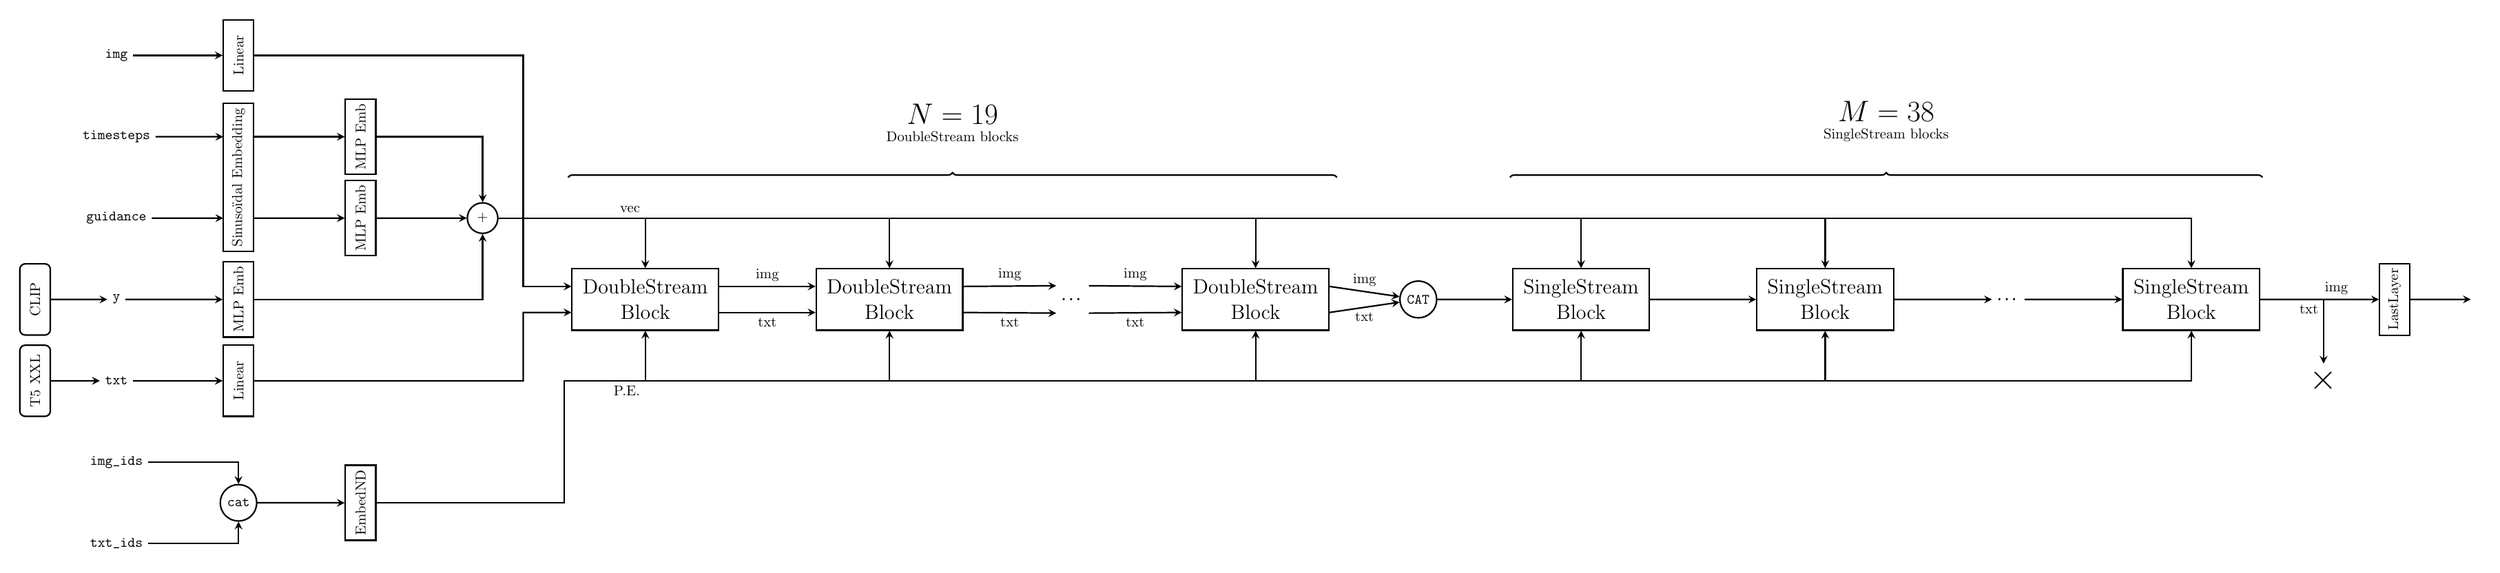
\begin{tikzpicture}[
    >=stealth,
    thick,
    scale=0.75,
    every node/.style={scale=0.75},
    block/.style={draw, rotate=90, minimum width=1.75cm, minimum height=.75cm},
    op/.style={draw, shape=circle, minimum width=.75cm}, % Operator (+, *, CAT...)
    stream/.style={draw, font=\Large, inner sep=7.5pt},
    align=center
]
    % INPUTS
    \node (in_img) at (0, 0) {\verb|img|};
    \node (in_timesteps) at (0, -2) {\verb|timesteps|};
    \node (in_guidance) at (0, -4) {\verb|guidance|};
    \node (in_y) at (0, -6) {\verb|y|}; % CLIP output
    \node (in_txt) at (0, -8) {\verb|txt|}; % T5XXL output
    \node (in_img_ids) at (0, -10) {\verb|img_ids|};
    \node (in_txt_ids) at (0, -12) {\verb|txt_ids|};

    % CLIP and T5 text encoders
    \node (CLIP) at (-2, -6) [block, rounded corners=.1cm] {CLIP}; % CLIP output
    \node (T5XXL) at (-2, -8) [block, rounded corners=.1cm] {T5 XXL}; % T5XXL output
    % Connect those to their output
    \draw[->] (CLIP) -- (in_y);
    \draw[->] (T5XXL) -- (in_txt);
    
    % INPUTS EMBEDDINGS
    \node (linear_01) at (3, 0) [block] {Linear};
    \node (sin_emb) at (3, -3) [block, minimum width=1.75*2cm] {Sinusoïdal Embedding};
    \node (mlp_emb_01) at (6, -2) [block] {MLP Emb};
    \node (mlp_emb_02) at (6, -4) [block] {MLP Emb};
    \node (mlp_emb_03) at (3, -6) [block] {MLP Emb};
    \node (vec_plus) at (9, -4) [op] {+};
    \node (linear_02) at (3, -8) [block] {Linear};
    \node (PE_cat) at (3, -11) [op] {\verb|cat|};
    \node (EmbedND) at (6, -11) [block] {EmbedND};
    
    % Connect inputs to embedding layers
    \draw[->] (in_img) -- (linear_01);
    \draw[->] (in_timesteps) -- ([xshift=-0.375cm]sin_emb |- in_timesteps);
    \draw[->] (in_guidance) -- ([xshift=-0.375cm]sin_emb |- in_guidance);
    \draw[->] ([xshift=0.375cm]mlp_emb_01 -| sin_emb) -- (mlp_emb_01);
    \draw[->] ([xshift=0.375cm]mlp_emb_02 -| sin_emb) -- (mlp_emb_02);
    \draw[->] (in_y) -- (mlp_emb_03);
    \draw[->] (mlp_emb_01) -| (vec_plus);
    \draw[->] (mlp_emb_02) -- (vec_plus);
    \draw[->] (mlp_emb_03) -| (vec_plus);
    \draw[->] (in_txt) -- (linear_02);
    \draw[->] (in_img_ids) -| (PE_cat);
    \draw[->] (in_txt_ids) -| (PE_cat);
    \draw[->] (PE_cat) -- (EmbedND);
    
    % DOUBLE STREAM BLOCKS
    \node (DoubleStream_01) at (13, -6) [stream] {DoubleStream\\Block};
    \node (DoubleStream_02) at (19, -6) [stream] {DoubleStream\\Block};
    \node (DoubleStream_dots) at (23.5, -6) [minimum height=1.5cm] {\textbf{\dots}};
    \node (DoubleStream_03) at (28, -6) [stream] {DoubleStream\\Block};
    
    % Connect embeddings to DS blocks
    \draw[->] (linear_01) -- ++(7, 0)  |- (DoubleStream_01.170);
    \draw[->] (linear_02) -- ++(7, 0)  |- (DoubleStream_01.190);
    
    % Connect DS blocks together
    \draw[->] (DoubleStream_01.10) -- node[above]{img} (DoubleStream_02.170);
    \draw[->] (DoubleStream_01.350) -- node[below]{txt} (DoubleStream_02.190);
    \draw[->] (DoubleStream_02.10) -- node[above]{img} (DoubleStream_dots.140);
    \draw[->] (DoubleStream_02.350) -- node[below]{txt} (DoubleStream_dots.220);
    \draw[->] (DoubleStream_dots.40) -- node[above]{img} (DoubleStream_03.170);
    \draw[->] (DoubleStream_dots.320) -- node[below]{txt} (DoubleStream_03.190);
    
    % Concat streams node between DS and SS nodes
    \node (streams_cat) at (32, -6) [op] {\verb|CAT|};
    \draw[->] (DoubleStream_03.10) --  node[above]{img} (streams_cat);
    \draw[->] (DoubleStream_03.350) --  node[below]{txt} (streams_cat);
    
    % SINGLE STREAM BLOCKS
    \node (SingleStream_01) at (36, -6) [stream] {SingleStream\\Block};
    \node (SingleStream_02) at (42, -6) [stream] {SingleStream\\Block};
    \node (SingleStream_dots) at (46.5, -6) [minimum height=1.5cm] {\textbf{\dots}};
    \node (SingleStream_03) at (51, -6) [stream] {SingleStream\\Block};
    
    % Connect SS blocks together
    \draw[->] (streams_cat) -- (SingleStream_01);
    \draw[->] (SingleStream_01) -- (SingleStream_02);
    \draw[->] (SingleStream_02) -- (SingleStream_dots);
    \draw[->] (SingleStream_dots) -- (SingleStream_03);
    
    % END OF THE STREAM CHAIN
    \node (last) at (56, -6) [block] {LastLayer};
    \node (cross) at (54.25, -8) {\Huge $\times$};
    \draw[->] (SingleStream_03) -- node[above right]{img} (last);
    \draw[->] (SingleStream_03) -| node[below left]{txt} (cross);
    \node (final) at (58, -6) {};
    \draw[->] (last) -- (final);
    
    % vec and PE connections to the stream blocks (double and single)
    \draw[->] (vec_plus) -| node[above left]{vec} (DoubleStream_01);
    \draw[->] (vec_plus) -| (DoubleStream_02);
    \draw[->] (vec_plus) -| (DoubleStream_03);
    \draw[->] (vec_plus) -| (SingleStream_01);
    \draw[->] (vec_plus) -| (SingleStream_02);
    \draw[->] (vec_plus) -| (SingleStream_03);
    \draw[->] (EmbedND)  -| ++(5, 3) -| node[below left]{P.E.} (DoubleStream_01);
    \draw[->] (EmbedND)  -| ++(5, 3) -| (DoubleStream_02);
    \draw[->] (EmbedND)  -| ++(5, 3) -| (DoubleStream_03);
    \draw[->] (EmbedND)  -| ++(5, 3) -| (SingleStream_01);
    \draw[->] (EmbedND)  -| ++(5, 3) -| (SingleStream_02);
    \draw[->] (EmbedND)  -| ++(5, 3) -| (SingleStream_03);

    % CURLY BRACES FOR NUMBER OF DS AND SS BLOCKS
    \draw[decoration={brace}, decorate] (11.1, -3) -- node[above, yshift=.75cm]{\huge $N = 19$\\DoubleStream blocks} (30, -3);
    \draw[decoration={brace}, decorate] (34.25, -3) -- node[above, yshift=.75cm]{\huge $M = 38$\\SingleStream blocks} (52.75, -3);
  \end{tikzpicture}
\end{document}